% !TeX spellcheck = en_GB
%\documentclass[handout]{beamer}\mode<presentation>{\usetheme{AMSCesenaPurpleAndGold}}
\documentclass[presentation]{beamer}\mode<presentation>{\usetheme{AMSCesenaPurpleAndGold}}
%%%%

\usepackage{sd-lab-final}
\usepackage{my-listings}
\usepackage{forloop}

\newcommand{\bs}[1]{\textbackslash{}#1}
\newcommand{\labN}{9}
\newcommand{\labGroup}{https://gitlab.com/pika-lab/courses/ds/ay2021}
\newcommand{\labRepo}{\labGroup/lab-\labN}

\title[L\labN{} -- Final]{L\labN{} -- Conclusions \& Future Works}
%
\subtitle[SD]{Distributed Systems / Technologies}
%
\author[Ciatto \and Omicini]
{\emph{Giovanni Ciatto} \and Andrea Omicini\\
	\texttt{giovanni.ciatto@unibo.it \and andrea.omicini@unibo.it}}
%
\institute[DISI, Univ. Bologna]
{Dipartimento di Informatica -- Scienza e Ingegneria (DISI)\\\textsc{Alma Mater Studiorum} -- Universit{\`a} di Bologna a Cesena}
%
\date[A.Y. 2020/2021]{Academic Year 2020/2021}

\setbeamercovered{transparent}

\AtBeginSection{
	\begin{frame}[c]\frametitle{Outline}
		% 		\begin{multicols}{2}
		\tableofcontents[sectionstyle=show/shaded, subsectionstyle=hide/hide, subsubsectionstyle=hide/hide]
		% 		\end{multicols}
	\end{frame}
}

\AtBeginSubsection{
	\begin{frame}[c]\frametitle{Next in Line\ldots}
		\begin{multicols}{2}
			\small
			\tableofcontents[sectionstyle=show/shaded, subsectionstyle=show/shaded, subsubsectionstyle=hide/hide]
		\end{multicols}
	\end{frame}
}

\begin{document}

%\\\\\\\\\\\\\\\\\\\\\
\frame{\titlepage}
%\\\\\\\\\\\\\\\\\\\\\

\section{Recap}

\begin{frame}
    \frametitle{What we did so far}

	So far we learned how to:
	%
	\begin{enumerate}
		\item[(L1)] \emph{automate} software building, testing, and dependency management
		\vfill 
		\item[(L2)] exploit \alert{agents} to govern the \emph{behavioural} dimension of software 
        \vfill 
		\item[(L3)] govern \emph{concurrent} systems via \alert{asynchronous programming}
        \vfill 
		\item[(L4)] \emph{build} agents on top of asynchronous and multi-threaded programming
		\vfill 
		\item[(L5)] exploit \alert{tuple spaces} to define the \emph{interactive} dimension of software 
		\vfill 
		\item[(L6)] \emph{build} tuple spaces on top of asynchronous programming 
		\vfill 
		\item[(L7)] \emph{model} \& reason about concurrent/distributed systems in an abstract and formal way
		\vfill 
		\item[(L8)] make tuple spaces \emph{distributed} via \alert{Web Services} 
		\vfill 
		\item[\textbf{(L9)}] exploit \emph{distributed tuple spaces} as a coordination medium for \alert{distributed agents}
    \end{enumerate}

\end{frame}

\section{Distributed Agents}

\subsection{Architecture}

\begin{frame}[allowframebreaks]
	\frametitle{Vision}

	\begin{center}
		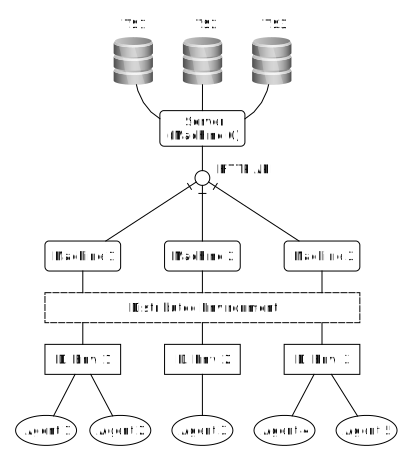
\includegraphics[height=0.8\textheight]{./img/overview.pdf}
	\end{center}

	\framebreak

	Explanation:
	%
	\medskip
	%
	\begin{itemize}
		\item at least $N + 1$ machines
		%
		\begin{itemize}
			\item one is the \linda{} server
			\item the others host agents
		\end{itemize}
		
		\medskip
		
		\item distributed \alert{environments} are available on each machine
		%
		\begin{itemize}
			\item letting agents exploit \alert{remote} tuple spaces
		\end{itemize}

		\medskip

		\item distributed environments may be split over multiple machines
		%
		\begin{itemize}
			\item all instances share the same \alert{environment name}, which is locally unique
		\end{itemize}

		\medskip

		\item agents running on some machine \alert{can interact} with agents running on other machines
		%
		\begin{itemize}
			\item because interaction is \alert{mediated} by tuple spaces
			\item and tuple spaces are \alert{distributed}
		\end{itemize}  
	\end{itemize}

	\framebreak

	\begin{alertblock}{Question}\centering
		How long does it take to realise this vision?
	\end{alertblock}
\end{frame}

\subsection{Implementation}

\begin{frame}[allowframebreaks]
	\frametitle{Realising the Vision -- Distributed Environments}

	Distributed Enviroments can be realised as follows:
	%
	\lstinputlisting[language=Java]{./code/DistributedEnvironment.java}

	\framebreak

	\begin{itemize}
		\item Assuming that the local implementation \alert{instantiates} tuple spaces via the method:
		%
		\begin{center}\ttfamily
			TextualSpace newTextualSpace(String name)
		\end{center}

		\smallskip
	
		\item The \alert{distributed} implementation simply overrides this method
		%
		\begin{itemize}
			\item changing the way tuple spaces are instantiated
			\item enforcing the creation of \alert{distributed} tuple spaces
		\end{itemize}

		\smallskip

		\item To create remote tuple spaces, the environment must know:
		%
		\begin{itemize}
			\item the \linda{} serivice's hostname and port
			\item[!] we assume these data are provided upon environment creation 
		\end{itemize}

		\smallskip

		\item Every time an agent running on a distributed environment requests a tuple space it gets a \alert{remote} tuple space
		%
		\begin{itemize}
			\item which actually stores tuples \emph{elsewhere}
			\item which is accessible from other machines as well
		\end{itemize}

		\smallskip

		\item Other agents running on other distributed environment, running on other machines may do the same thing
	\end{itemize}

	\framebreak

	The environment interface is extended accordingly with static factories:
	%
	\lstinputlisting[language=Java]{./code/Environment.java}
\end{frame}

\begin{frame}[allowframebreaks]
	\frametitle{Realising the Vision -- Deployment}

	Finally,
	%
	\medskip
	%
	\begin{itemize}
		\item we need some means to \alert{start} a distributed environment instance
		%
		\begin{itemize}
			\item on a standalone \alert{process}
			\item possibly running on a standalone \alert{machine}
		\end{itemize}

		\medskip

		\item we also need some means to start all the agents that should run locally, within that process
		
		\medskip

		\item[!] and ordinary Java \texttt{main} will be ok for the purpose
		%
		\begin{itemize}
			\item we can assume some information are provided as arguments, e.g.
			%
			\begin{itemize}
				\item the environment name (shared among several processes)
				\item the \linda{} service host name \& port
			\end{itemize}
		\end{itemize}
		
		\framebreak

		\item[!] we also need some means to guarantee the service is started \alert{before} other processes
		%
		\begin{itemize}
			\item process (re)starting order is a complicate matter of \emph{deploy}
			\item we won't cover it in this course
			\item \alert{orchestration} tools like \texttt{Docker Swarm} or \texttt{Kubernetes} may be useful to the purpose
		\end{itemize} 

	\end{itemize}

	\framebreak

	A simple entry point for distributed environment and their local agents:
	%
	\lstinputlisting[language=Java,morekeywords={var}]{./code/Main.java}

	\framebreak

	Deployment order:
	%
	\medskip
	%
	\begin{enumerate}
		\item launch the \linda{} service on port $P$ on some host $H$
		\medskip
		\item launch the \emph{first} instance of the distributed environment named $N$
		%
		\begin{itemize}
			\item passing $H$, $P$, and $N$ as arguments to its \texttt{Main}
		\end{itemize}
		\medskip
		\item launch the \emph{second} instance of the distributed environment named $N$
		%
		\begin{itemize}
			\item passing $H$, $P$, and $N$ as arguments to its \texttt{Main}
		\end{itemize}
		\medskip
		\item[$\vdots$]
	\end{enumerate}

\end{frame}

\subsection{Instant Messaging Example}

\startDemo

\begin{frame}[allowframebreaks]
	\frametitle{Demo \currentDemo{} -- Instant Messaging Example}

	\begin{enumerate}
		\item Consider the Lab-\labN{} repository on GitLab
		%
		\begin{center}
			\url{\labRepo}
		\end{center}

		\medskip

		\item Have a look to the new-entry behaviours in \texttt{sd.lab.agency.behaviour.impl.*}:
		%
		\begin{description}
			\item[\texttt{Send}] lets an agent send a message to another agent
			\item[\texttt{Receive}] lets an agent selectively receive a message
			\item[\texttt{ReadLine}] lets an agent read a line from an \texttt{InputStream}
			%
			\begin{itemize}
				\item[eg] \texttt{System.in}
			\end{itemize} 
		\end{description}

		\medskip

		\item Consider the \texttt{sd.lab.im.*} package, coming with 2 classes:
		%
		\begin{description}
			\item[\texttt{ChatterAgent}] implementing an agent aimed at letting human user chat with each others
			\item[\texttt{Chat}] is the entrypoint of a distributed environment containing one single \texttt{ChatterAgent}  
		\end{description}

		\medskip

		\item Each \texttt{ChatterAgent} represents (and is named after) a human user
		%
		\begin{itemize}
			\item it knows the \alert{name} of the person to chat with since its birth
			\item after its start it keeps consuming lines of text from \texttt{System.in} and send them to the other agent
			%
			\begin{itemize}
				\item if a line starts with \texttt{`:end'} it stops
			\end{itemize}
			\item after its start it keeps listening for messages from the other agent 
			%
			\begin{itemize}
				\item whenever a new message is received, it is printed on the local \texttt{System.out}
			\end{itemize}
		\end{itemize}

		\framebreak

		\item Can you guess how many lines of code are required to implement \texttt{ChatterAgent}?
		
		\framebreak

		\item $\sim40$ lines of Java code:
		%
		\lstinputlisting[language=Java]{./code/ChatterAgent.java}
	\end{enumerate}

	\begin{alertblock}{Takeaway}\centering
		The code is compact because the abstraction level is adequate
	\end{alertblock}

	\framebreak

	\begin{block}{Gradle tasks to start the demo}
		\begin{description}
			\item[\texttt{./gradlew \textit{service} -P\textit{port}=PORT}] 
			starts the \linda{} service on \texttt{localhost:PORT}  
			%
			\begin{itemize}
				\item default \texttt{PORT} is \texttt{8080}
			\end{itemize}

			\item[\texttt{./gradlew \textit{chatter} -P\textit{host}=H -P\textit{port}=P -P\textit{me}=M -P\textit{other}=O}]
			starts \emph{(i)} a distributed environment named \texttt{`sd.lab.im.Chat'} which assumes the \linda{} service is running on \texttt{H:P}, and \emph{(ii)} a \texttt{ChatterAgent} named \texttt{M} which is willing to chat with an agent named \texttt{O}
			%
			\begin{itemize}
				\item default \texttt{H} is \texttt{localhost}
				\item default \texttt{P} is \texttt{8080}
			\end{itemize}
		\end{description}
	\end{block}

	\begin{exampleblock}{Running the demo}
		Using \alert{3 different shells}:
		%
		\begin{enumerate}
			\item \texttt{./gradlew service} 
			\item \texttt{./gradlew chatter -Pme=giovanni -Pother=andrea} 
			\item \texttt{./gradlew chatter -Pme=andrea -Pother=giovanni} 
		\end{enumerate}
	\end{exampleblock}
\end{frame}

\section{Next Steps}

\subsection{Overview}

\begin{frame}{Overview}

	\begin{itemize}
		\item We have finally completed our mini agent-based framework for distributed systems
		%
		\begin{itemize}
			\item and lab activity
		\end{itemize}

		\vfill

		\item Yet, several features are currently missing to make our framework actually mature
		%
		\begin{itemize}
			\item[eg] \fipa{} interaction protocols
			\item[eg] a white-pages services, a.k.a. naming service
			\item[eg] a yellow-pages services 
			\item[eg] some access control mechanism for the \linda{} service 
			\item[eg] the exploitation of \emph{Web Sockets} for handling \linda{}'s suspensive semantics via Web
		\end{itemize}

		\vfill

		\item Consider each feature an \alert{optional}, unconstrained exercise you can perform to deepen your understanding
		%
		\begin{itemize}
			\item further material can be provided on demand for each topic
		\end{itemize}
	\end{itemize}
\end{frame}

\startExercise

\subsection{\fipa{} Interaction Protocols}

\begin{frame}[allowframebreaks]
\frametitle{Exercise \currentExercise{} -- \fipa{} Interaction Protocols (IP)}
	\begin{alertblock}{This is an \textbf{optional}, \textbf{unconstrained} exercise}
		\begin{itemize}
			\item do it if you want to deepen your understanding
			\item you are free to design your solution as you prefer
			\item no test is provided
		\end{itemize}
	\end{alertblock}

	\begin{block}{Motivation}
		\begin{itemize}
			\item Send and Receive behaviours, as well as \linda{} primitives, are \alert{basic} interaction mechanisms
			\item Agents often compose them into more complex \alert{interaction protocols}
			\item Interaction protocols are design patterns for interaction 
			\item A rich agent framework should include some API (ie behaviours) for IP
		\end{itemize}
	\end{block}

	\begin{block}{Goal}
		\begin{itemize}
			\item Design and implement some composite behaviours for agents, supporting \fipa{} IP
			%
			\item Detailed specification here: \url{http://www.fipa.org/repository/standardspecs.html}
			%
			\item[eg] Request, Query, Contract Net, Subscribe, \ldots
		\end{itemize}
	\end{block}

	\begin{exampleblock}{Hint}
		\begin{itemize}
			\item consider mimicking \jade{}'s IP behaviour classes
		\end{itemize}
	\end{exampleblock}
\end{frame}

\startExercise

\subsection{The White-Pages Service}

\begin{frame}[allowframebreaks]
\frametitle{Exercise \currentExercise{} -- The White-Pages Service}
	\begin{alertblock}{This is an \textbf{optional}, \textbf{unconstrained} exercise}
		\begin{itemize}
			\item do it if you want to deepen your understanding
			\item you are free to design your solution as you prefer
			\item no test is provided
		\end{itemize}
	\end{alertblock}

	\begin{block}{Motivation}
		\begin{itemize}
			\item Agents in a distributed environment should not be assumed to know each others
			\item Agents should be able to discover each others dynamically
			\item A service keeping track of the AIDs of all agents is required
		\end{itemize}
	\end{block}

	\begin{block}{Goal}
		\begin{itemize}
			\item Design a distributed white-pages service keeping track of the AIDs of all the agents currently running within a distributed system
			\item Agents should be automatically registered upon startup \& deregistered before termination
			%
			\begin{itemize}
				\item[!] regardeless of what agent programmers do
			\end{itemize}
			\item Agents should be able to query the service whenever they want to discover the AIDs other agents running within the same distributed environment, possibly on different processes/machines
		\end{itemize}
	\end{block}

	\begin{exampleblock}{Hint}
		\begin{itemize}
			\item consider mimicking \jade{}'s AMS, at least at a functional level
			\item consider leveraging distributed tuple spaces to store AIDs 
		\end{itemize}
	\end{exampleblock}
\end{frame}

\startExercise

\subsection{The Yellow-Pages Service}

\begin{frame}[allowframebreaks]
\frametitle{Exercise \currentExercise{} -- The Yellow-Pages Service}
	\begin{alertblock}{This is an \textbf{optional}, \textbf{unconstrained} exercise}
		\begin{itemize}
			\item do it if you want to deepen your understanding
			\item you are free to design your solution as you prefer
			\item no test is provided
		\end{itemize}
	\end{alertblock}

	\begin{block}{Motivation}
		\begin{itemize}
			\item When looking for collaborations, agents may require to discover other agents\ldots
			\item \ldots on the basis of the services they can offer
			\item rather than their names
		\end{itemize}
	\end{block}

	\begin{block}{Goal}
		\begin{itemize}
			\item Design a distributed yellow-pages service keeping track of \alert{service descriptor} of all the agents willing to offer a service
			
			\item Agents should be able to (de)register whenever they want

			\item Agents should be able to query the service whenever they want to discover service descriptor of other agents running within the same distributed environment, possibly on different processes/machines
		\end{itemize}
	\end{block}

	\begin{exampleblock}{Hint}
		\begin{itemize}
			\item consider mimicking \jade{}'s DF, at least at a functional level
			\item consider leveraging distributed tuple spaces to store service descriptors 
		\end{itemize}
	\end{exampleblock}
\end{frame}

\startExercise

\subsection{Access Control for \linda{} WS}

\begin{frame}[allowframebreaks]
\frametitle{Exercise \currentExercise{} -- Access Control for \linda{} WS}
	\begin{alertblock}{This is an \textbf{optional}, \textbf{unconstrained} exercise}
		\begin{itemize}
			\item do it if you want to deepen your understanding
			\item you are free to design your solution as you prefer
			\item no test is provided
		\end{itemize}
	\end{alertblock}

	\begin{block}{Motivation}
		\begin{itemize}
			\item The \linda{} WS is very trivial: no \alert{access control} (AC) is performed on clients
			\item Users are not explicitly represented as resources
			\item Buggy or misbehaving agents may alter the correct functioning of a MAS 
		\end{itemize}
	\end{block}

	\begin{block}{Goal}
		\begin{itemize}
			\item Design some AC mechanism for \linda{} tuple spaces
			
			\item Extend the \linda{} WS accordingly

			\item Exploit authentication tokens (e.g. JWT) to handle authentication \& authorization at the HTTP level
			
			\item Extend \texttt{RemoteTupleSpace}s to support authentication
		\end{itemize}
	\end{block}

	\begin{exampleblock}{Hint}
		\begin{itemize}
			\item consider consulting the additional material on this topic
		\end{itemize}
	\end{exampleblock}
\end{frame}

\startExercise

\subsection{Suspensive Semantics via Web Sockets}

\begin{frame}[allowframebreaks]
\frametitle{Exercise \currentExercise{} -- Suspensive Semantics via Web Sockets}
	\begin{alertblock}{This is an \textbf{optional}, \textbf{unconstrained} exercise}
		\begin{itemize}
			\item do it if you want to deepen your understanding
			\item you are free to design your solution as you prefer
			\item no test is provided
		\end{itemize}
	\end{alertblock}

	\begin{block}{Motivation}
		\begin{itemize}
			\item We currently implement suspensive semantics over HTTP via \alert{long polling}
			\item This is inadequate for modern WS
			\item Web sockets should be used instead
		\end{itemize}
	\end{block}

	\begin{block}{Goal}
		\begin{itemize}
			\item Explore how Web Sockets work in general
			\item Explore how Web Sockets work in Javalin and Java's HTTP API
			\item Use Web Sockets instead of long polling within the \linda{} Works
			\item Modify \texttt{RemoteTupleSpace}s accordingly
		\end{itemize}
	\end{block}

	\begin{exampleblock}{Hint}
		\begin{itemize}
			\item consider consulting the additional material on this topic
		\end{itemize}
	\end{exampleblock}
\end{frame}

%===============================================================================
\section*{}
%===============================================================================

%\\\\\\\\\\\\\\\\\\\\\
\frame{\titlepage}
%\\\\\\\\\\\\\\\\\\\\\

%%===============================================================================
%\section*{\refname}
%%===============================================================================
%
%%\\\\\\\\\\\\\\\\\\\\\
%%%%%
%%\begin{frame}[t,allowframebreaks]\scriptsize
%\begin{frame}[c]\footnotesize
%\frametitle{\refname}
%\bibliographystyle{apalike}
%\bibliography{sd-lab-jadelike-agents}
%\end{frame}
%%\\\\\\\\\\\\\\\\\\\\\

%%%%%%%%%%%%%%%%%%%%%%%%%%%%%%%%%%%%%%%%%%%%%%%%%%%%%%%%%%%%%%%%%%%%%%%%%%%%%%%
\end{document}
%%%%%%%%%%%%%%%%%%%%%%%%%%%%%%%%%%%%%%%%%%%%%%%%%%%%%%%%%%%%%%%%%%%%%%%%%%%%%%%%

